\section
[$M(n)/M(n)/1$ Queue]
{$\mathbf{M(n)/M(n)/1}$ Queue}
\label{sec:mnmn1}

\subsection*{Theory and Exercises}

\Opensolutionfile{hint}
\Opensolutionfile{ans}

As it turns out, many more single-server queueing situations can be
modeled and analyzed by making a judicious choice of $\lambda(n)$ and
$\mu(n)$ in~\eqref{eq:25}, to wit,
$ \lambda(n) p(n) = \mu(n+1)p(n+1)$. For these queueing systems we
just present the results. In the exercises we ask you to derive the
formulas---the main challenge is not to make computational errors. 

It is important to realize that the interarrival times and service times need to be memoryless for the analysis below; the rates, however, may  depend on the number of the jobs in the system. Specifically, consider the departure time $D_k$ of the $k$th job, so that $A_{A(D_k)+1}$ is the arrival time of the next job. If $L(D_k)=n$, then we require that for every $k$ 
\begin{equation*}
  \P{A_{A(D_k)+1} - D_k \leq x} = 1-e^{-f(n) \lambda x},
\end{equation*}
for some function $f:\N\to [0,\infty)$. Next, since $D_{D(A_k)+1}$ is the time until the next departure after $A_k$, we assume for all $k$,
\begin{equation*}
  \P{D_{D(A_k)+1} - A_k \leq x} = 1-e^{-g(n) \mu x},
\end{equation*}
if $L(A_k)=n$ (not $L(A_k-)=n$) for some function $g:\N \to [0,\infty)$. 


For the $M/M/1/K$, i.e., a system that cannot contain more than $K$ jobs, take
  \begin{align*}
    \lambda(n) &= 
  \begin{cases}
    \lambda, &\text{ if } n < K, \\
    0, &\text{ if } n \geq K, \\
  \end{cases} \\
\mu(n) &= \mu.
  \end{align*}

\begin{exercise} ($M/M/1/K$ queue)
 Derive 
\begin{subequations}\label{eq:8}
 \begin{align}
p(n) &=  \frac{\rho^n}G, \quad 0\leq n \leq K,\\
G &= \frac{1-\rho^{K+1}}{1-\rho}, \text{ (normalization constant)},\\
P_{\text{loss}} &= \P{L=K} = \frac{\rho^K}G = \frac{1-\rho}{1-\rho^{K+1}} \rho^K.
\end{align}
\end{subequations}
\begin{hint}
  Use the equations around~\eqref{eq:38}.
\end{hint}
  \begin{solution}
Note that 
\begin{equation*}
1 = \sum_{i=0}^K p(i) = p(0)\sum_{i=0}^K \rho^i  = p(0) \frac{1-\rho^{K+1}}{1-\rho}. 
\end{equation*}
Thus, for the normalization constant $G$ we take 
\begin{equation*}
G=\frac 1{p(0)} = \frac{1-\rho^{K+1}}{1-\rho},
\end{equation*}
and the result follows. 
  \end{solution}
\end{exercise}

\begin{exercise} 
   Show that as $K\to\infty$, the performance measures of the $M/M/1/K$ converge to those of the $M/M/1$ queue. 
  \begin{hint}
Use that $\sum_{i=0}^n x^i = (1-x^{n+1})/(1-x)$. BTW, is it
    necessary for this expression to be true that $|x|<1$? What should
    you require for $|x|$ when you want to take the limit
    $n\to\infty$?
  \end{hint}
  \begin{solution}
To take the limit $K\to\infty$---mind, not the limit $n\to\infty$---, write
\begin{equation*}
G= \frac{1-\rho^{K+1}}{1-\rho} = \frac{1}{1-\rho} -\frac{\rho^{K+1}}{1-\rho}.
\end{equation*}
Since $\rho^{K+1}\to 0$ as $K\to \infty$ (recall, $\rho<1$),  we get
\begin{equation*}
G \to \frac{1}{1-\rho}, 
\end{equation*}
as $K\to\infty$.  Therefore $p(n)=\rho^n/G \to \rho^n(1-\rho)$, and
the latter are the steady-state probabilities of the $M/M/1$
queue. Finally, if the steady state probabilities are the same, the
performance measures (which are derived from $p(n)$) must be the same.
  \end{solution}
\end{exercise}


For the $M/M/c$ queue we can take
  \begin{align*}
\lambda(n) &= \lambda, \\
    \mu(n) &= 
  \begin{cases}
    n\mu, &\text{ if } n \leq c, \\
    c\mu, &\text{ if } n \geq c.
  \end{cases}
  \end{align*}
This model is also known as the \recall{Erlang $C$}-formula. 

\begin{exercise}($M/M/c$)
Define the load as 
\begin{subequations}\label{eq:9}
\begin{equation}
  \rho = \frac{\lambda}{c\mu}.
\end{equation}
  Then, derive
 \begin{align}
p(n) &= \frac{1}G \frac{(c\rho)^n}{n!}, \quad n=0,\ldots, c, \label{eq:502}\\
p(n) &= \frac{1}G \frac{c^c\rho^n}{c!}, \quad n=c,c+1, \ldots \\
G &=\sum_{n=0}^{c-1} \frac{(c\rho)^n}{n!} + \frac{(c\rho)^c}{(1-\rho)c!}, \label{eq:501}\\
\E{L_Q} &= \sum_{n=c}^\infty (n-c) p(n) = \frac{(c\rho)^c}{c! G}\frac{\rho}{(1-\rho)^2}, \\ 
\E{L_S} &= \sum_{n=0}^{c}n p(n) + \sum_{n=c+1}^\infty c p(n) = \frac{\lambda}\mu.
\end{align}
\end{subequations}
  \begin{hint}
 Use $\lambda(n)p(n) = \mu(n+1)p(n+1)=\min\{c, n+1\}\mu p(n+1)$.
  \end{hint}

  \begin{solution}
First we use the hint to  establish a generic relation for $p(n+1)$:
    \begin{align*}
       p(n+1) 
&= \frac{\lambda}{\mu(n+1)}p(n) 
= \frac{\lambda}{\min\{c, n+1\} \mu }p(n) \\
&= \frac{1}{\min\{c, n+1\}}\frac\lambda\mu p(n) 
= \frac{1}{\min\{c, n+1\}}(c\rho) p(n) \\
&= \frac{1}{\min\{c, n+1\}\min\{c, n\}}(c\rho)^2 p(n-1) 
= \frac{1}{\Pi_{k=1}^{n+1}\min\{c, k\}}(c\rho)^{n+1} p(0).
    \end{align*}
Thus, if $n<c$:
\begin{equation*}
  p(n) = \frac{1}{\Pi_{k=1}^{n}\min\{c, k\}}(c\rho)^{n} p(0) = \frac{(c\rho)^n}{n!} p(0),
\end{equation*}
since $\min\{c,k\}=k$ when $k<c$. If $n\geq c$:
\begin{align*}
  p(n) 
&= \frac{1}{\Pi_{k=1}^{n}\min\{c, k\}}(c\rho)^{n} p(0) \\
&= \frac{1}{\Pi_{k=1}^{c-1} k \cdot \Pi_{k=c}^{n} c}(c\rho)^{n} p(0) \\
&= \frac{1}{(c-1)! c^{n-c+1}}c^n\rho^{n} p(0) \\
&= \frac{1}{c! c^{n-c}}c^n\rho^{n} p(0) = \\
&= \frac{c^c}{c!}\rho^{n} p(0).
\end{align*}


To obtain  the normalization constant $G$,
\begin{align*}
1 &= \sum_{n=0}^\infty p(n) 
= \sum_{n=0}^{c-1} p(n) + \sum_{n=c}^\infty p(n) \\
&=p(0) \sum_{n=0}^{c-1}\frac{(c\rho)^n}{n!} + 
 p(0)\sum_{n=c}^{\infty} \frac{c^c}{c!} \rho^{n}  \\
&=p(0)\sum_{n=0}^{c-1}\frac{(c\rho)^n}{n!} + 
 p(0) \sum_{n=c}^{\infty} \frac{(c\rho)^c}{c!} \rho^{n-c}  \\
&= 
p(0)\sum_{n=0}^{c-1}\frac{(c\rho)^n}{n!} + 
p(0)\frac{(c\rho)^c}{c!} \sum_{n=0}^{\infty} \rho^n \\
&= 
p(0) \sum_{n=0}^{c-1}\frac{(c\rho)^n}{n!} + 
p(0)\frac{(c\rho)^c}{c!(1-\rho)}.
\end{align*}
Hence, by setting
\begin{equation*}
  G= \sum_{n=0}^{c-1}\frac{(c\rho)^n}{n!} + \frac{(c\rho)^c}{c!(1-\rho)},
\end{equation*}
we get $p(0)=1/G$, and from this the rest follows. 

Next, 
\begin{align*}
  \E{L_Q} 
&=\sum_{n=c}^\infty (n-c) p(n) \\
&=\sum_{n=c}^\infty (n-c) \frac{c^c}{c!}\rho^{n} p(0) \\
&=\frac{c^c\rho^c}{G c!} \sum_{n=c}^\infty (n-c) \rho^{n-c} \\
&=\frac{c^c\rho^c}{G c!} \sum_{n=0}^\infty n \rho^n 
=\frac{c^c\rho^c}{G c!} \frac{\rho}{(1-\rho)^2},
\end{align*}
where, with our common trick (if we don't want to use generating functions),
\begin{align*}
  \sum_{n=0}^\infty n \rho^n 
&= \sum_{n=0}^\infty \sum_{i=1}^\infty \1{i\leq n} \rho^n
= \sum_{i=1}^\infty   \sum_{n=0}^\infty \1{i\leq n} \rho^n\\
&= \sum_{i=1}^\infty   \sum_{n=i}^\infty \rho^n
= \sum_{i=1}^\infty   \rho^i \sum_{n=0}^\infty \rho^n\\
&= \frac1{1-\rho} \sum_{i=1}^\infty   \rho^i 
= \frac\rho{1-\rho} \sum_{i=0}^\infty   \rho^i 
= \frac\rho{(1-\rho)^2}.
\end{align*}
Observe again that using indicators and Fubini's theorem
(interchanging summations and integrals) makes the above computation
painless. Realize, by the way, that
\begin{equation*}
  \sum_{n=0}^\infty n p(n) = \sum_{n=1}^\infty n p(n).
\end{equation*}

We next show that the expected number of jobs in service is given
by
    \begin{equation*}
      \E{L_S} = \sum_{n=0}^{c} n p(n) + \sum_{n=c+1}^{\infty} c p(n).
    \end{equation*}
    This expression is not the easiest to start with. With a slight
    modification the entire derivation becomes easier. I also pre-multiply by the normalization constant $G$ to get rid of it on the right hand side. 
    \begin{align*}
      G \E{L_S}
&= G \sum_{n=0}^{c} n p(n) + \sum_{n=c+1}^{\infty} c p(n) \\
&= \sum_{n=1}^{c} n \frac{(c\rho)^n}{n!}  + \sum_{n=c+1}^{\infty} c \frac{c^c\rho^n}{c!} 
= \sum_{n=1}^{c} \frac{(c\rho)^n}{(n-1)!}  + \frac{c^{c+1}}{c!}\sum_{n=c+1}^{\infty} \rho^n\\
&= \sum_{n=0}^{c-1} \frac{(c\rho)^{n+1}}{n!}  + \frac{(c\rho)^{c+1}}{c!}\sum_{n=0}^{\infty} \rho^n
= c\rho \left(\sum_{n=0}^{c-1} \frac{(c\rho)^n}{n!}  + \frac{(c\rho)^{c}}{c!(1-\rho)}\right).
    \end{align*}
Observe that the right hand side is precisely equal to $\rho c G$, and hence,
\begin{equation*}
  \E{L_S} = c\rho = \frac\lambda\mu.
\end{equation*}
\end{solution}
\end{exercise}

\begin{exercise}
  Check that  Eq.\eqref{eq:9} for the $M/M/c$ queue reduces to the $M/M/1$ queue if $c=1$.
  \begin{hint}
Fill in $c=1$. Realize that this is a check on the formulas.
  \end{hint}
  \begin{solution}
Take $c=1$
\begin{subequations}
 \begin{align}
p(0) &= \frac{1}G \frac{(c\rho)^0}{0!}=\frac1 G, \quad n=0,\ldots, 1-1 \\
p(n) &= \frac{1}G \frac{c^c\rho^n}{c!} = \frac{1}G \frac{1^1\rho^n}{1!} =\frac{\rho^n}G , \quad n=1,1+1, \ldots \\
G &=\sum_{n=0}^{c-1} \frac{(c\rho)^n}{n!} + \frac{(c\rho)^c}{(1-\rho)c!}
=\sum_{n=0}^{0} \frac{\rho^0}{0!} + \frac{\rho}{(1-\rho)} = 1 + \frac{\rho}{1-\rho} = \frac1{1-\rho}
\\
\E{L_Q} &= \frac{(c\rho)^c}{c! G}\frac{\rho}{(1-\rho)^2} = 
= \frac{\rho}{1/(1-\rho)}\frac{\rho}{(1-\rho)^2} = \frac{\rho^2}{1-\rho} \\
\E{L_S} &= \sum_{n=0}^{c}n p(n) + \sum_{n=c+1}^\infty c p(n) = p(1) + 1 \sum_{n=2}^\infty p(n) = 1- p(0) = \rho.
\end{align}
\end{subequations}
Everything is in accordance to the formulas we derived earlier for the $M/M/1$ queue.    
  \end{solution}
\end{exercise}


From this we can easily get the $M/M/c/c$ queue; here jobs cannot be
in queue, only in service, and the system has $c$ servers.  This model
is also known as the Erlang $B$-formula and is often used to determine
the number of beds at hospitals, where the beds act as servers and the
patients as jobs.

\begin{exercise}($M/M/c/c$)
  Find $\lambda(n)$ and $\mu(n)$ for the $M/M/c/c$ queue, and determine the performance measures.
  \begin{solution} Take,
    $\lambda(n) = \lambda$ if $n< c$, and $\lambda(n)=0$ for $n\geq c$. Also, let, $\mu(n) = n \mu$ for $n\leq c$. (And $n$ can never be larger than $c$, since $\lambda(n) = 0$ for $n\geq c$.) Define $\rho = \lambda/c \mu$. Then, we see that $p(n) = p(0)(c\rho)^n/n!$. For the normalization
    \begin{equation*}
      1=\sum_{n=0}^c p(n) = p(0) \sum_{n=0}^c \frac{(c\rho)^n}{n!}.
    \end{equation*}
Thus,  the normalization constant $G=\sum_{n=0}^{c}$, and $p(0)=G^{-1}$. 

Since there are as many servers as places available in the system, $\E{L_Q}=0$. The expected number of servers busy is
    \begin{align*}
      \E{L_S} 
&= \sum_{n=0}^{c} n p(n) = G^{-1} \sum_{n=0}^c n \frac{(\lambda/\mu)^n}{n!} \\
&= G^{-1} \sum_{n=1}^c n \frac{(\lambda/\mu)^n}{n!} = \frac{\lambda}{\mu G} \sum_{n=0}^{c-1} \frac{(\lambda/\mu)^{n}}{(n)!} \\
&= \frac{\lambda}{G\mu} \left(G- \frac{(\lambda/\mu)^c}{c!}\right).
    \end{align*}
  \end{solution}
\end{exercise}

\begin{exercise}
Consider the $M/M/2/3$ queue with arrival rate $\lambda$ and
service rate $\mu$ (thus, at most 2 jobs can be in service and 1 in queue.)
 Derive first the level-crossing equations for this queueing system, then  derive a simple and closed form expressions for the state    probabilities in steady state. 
  \begin{hint}
 Think about what would be the appropriate model choices for
   $\lambda(n)$ and $\mu(n)$ and use the level-crossing equations
   $\lambda(n) p(n) = \mu(n+1)p(n+1)$.  For instance, realize that
   $\lambda(3)=0$: the system cannot contain more than 3 jobs, hence a
   state with $4$ jobs must be impossible. We can achieve that by
   setting $\lambda(3)=0$. For the service rate, how many servers are
   busy when the system contains 2 or more jobs?  What does this say
   about $\mu(k)$ for $k=2$ or $k=3$.
  \end{hint}
  \begin{solution}
 Use the figure below. Make sure you understand why $\mu(2)=2\mu$ and so on. 
    \begin{center}
\begin{tikzpicture}[->,>=stealth',shorten >=1pt,auto,node distance=1.8cm,
                    semithick]
  \node[state] (0) {$p(0)$} ;
  \node[state] (1) [right of=0] {$p(1)$};
  \node[state] (2) [right of=1] {$p(2)$};
  \node[state] (3) [right of=2] {$p(3)$};

\path 
 (0) edge [bend left] node {$\lambda$} (1)
 (1) edge [bend left] node {$\mu$} (0)
 (1) edge [bend left] node {$\lambda$} (2)
 (2) edge [bend left] node {$2\mu$} (1)
 (2) edge [bend left] node {$\lambda$} (3)
 (3) edge [bend left] node {$2\mu$} (2);
\end{tikzpicture}
      
    \end{center}

From this figure it follows right away that:
    \begin{align*}
   \lambda p(0) &= \mu p(1) \\
   \lambda p(1)  &= 2\mu p(2) \\
   \lambda p(2)  &= 2\mu p(3)\\
    \end{align*}

Then,  from the above, with $\rho=\lambda/\mu$: 
    \begin{align*}
      p(1) &= \rho p(0), \\
      p(2) &= (\rho/2) p(1) = (\rho^2/2) p(0), \\
      p(3) &= (\rho/2) p(2) = (\rho^3/4) p(0).
    \end{align*}
Now we normalize to find $p(0)$. Thus, we want that:
\begin{equation*}
  1 = p(0)+p(1)+p(2)+p(3) = p(0)\left(1 + \rho + \frac{\rho^2}2 + \frac{\rho^3}4\right),
\end{equation*}
hence,
\begin{equation*}
p(0) = (1+\rho + \rho^2/2 + \rho^3/4)^{-1}.
\end{equation*}
   \end{solution}
\end{exercise}


\begin{exercise}(Multi-server queue with blocking) Consider the
  $M/M/c/c+K$ queue in which at most $c$ jobs can be in service and $K$ in queue. Try to derive the steady state probabilities
  $p(0)$, $p(1), \ldots$. You do not have to compute the normalization
  constant $G$. 
  \begin{hint}
Use $\lambda(n) p(n) = \mu(n+1)p(n+1)$ and
    find suitable expressions for $\lambda(n)$ and $\mu(n+1)$. 
  \end{hint}
  \begin{solution}
    $\lambda(n) \equiv \lambda$ for all $n<c+K$. When $n=c+K$,
    $\lambda(n)=0$, since then the system is full, and all arriving
    jobs will be dropped; in other words, there will still be jobs
    arriving to the system when $L=c+K$, but these jobs will be
    rejected, hence cannot generate a transition from state $c+K$ to
    $c+K+1$.  When $n<c$, $\mu(n)=n \mu$ since only $n$ servers
    are active/occupied when the system contains $n$ jobs. When
    $n\geq c$, $\mu(n) = c \mu$. Thus, using $\rho=\lambda/(c\mu)$, for $n<c$,
     \begin{equation*}
      p(n) = \frac{\lambda}{n\mu} p(n-1) = \frac{(\lambda/\mu)^n}{n!} p(0)=\frac{(c\rho)^n}{n!}p(0).
     \end{equation*}
For $c\leq n\leq c+K$ and using the above to get $p(c-1)$:
 \begin{align*}
 p(n) &= \frac{\lambda}{c\mu} p(n-1) 
= \rho p(n-1) = \rho^2 p(n-2) = \ldots\\
&=\rho^{n-c+1} p(c-1) 
=\rho^{n-c+1} \frac{(c\rho)^{c-1}}{(c-1)!}p(0)\\
&=\rho^{n} \frac{(c)^{c-1}}{(c-1)!}p(0) 
=\rho^{n} \frac{(c)^{c-1}c}{(c-1)!c}p(0) =\frac{c^c \rho^n}{c!} p(0).
 \end{align*}
The normalization is trivial, numerically at least.
  \end{solution}
\end{exercise}


From the $M/M/c$ queue (or the $M/M/c/c$ queue) we can also obtain the
$M/M/\infty$, i.e., a queueing system with ample servers. By taking
the limit $c\to\infty$, note first that in~(\ref{eq:501}),
\begin{equation*}
\frac{(c\rho)^c}{(1-\rho)c!} = \frac{(\lambda/\mu)^c}{(1-\rho)c!}\to 0, \quad\text{as } c\to \infty.
\end{equation*}
Hence
\begin{equation*}
G =\sum_{n=0}^{c-1} \frac{(c\rho)^n}{n!} + \frac{(c\rho)^c}{(1-\rho)c!} \to \sum_{n=0}^{\infty} \frac{(c\rho)^n}{n!} = e^{\lambda/\mu}.
\end{equation*}
Next, for $n\geq c$:
\begin{equation*}
  p(n) = \frac{1}G \frac{c^c\rho^n}{c!} =\frac{\rho^n}{G}\frac{c^c}{c!} \to 0, 
\quad\text{as } c\to\infty,
\end{equation*}
since, from a standard limit $n^n/n! \to 0$ as $n\to\infty$. Therefore, for $n<c$: 
\begin{equation*}
  p(n) = \frac{1}G \frac{(c\rho)^n}{n!} = \frac{1}G \frac{(\lambda/\mu)^n}{n!} 
\to e^{-\lambda/\mu}  \frac{(\lambda/\mu)^n}{n!}, \quad\text{as } c\to\infty.
\end{equation*}
We see that the number of busy servers in the $M/M/\infty$ queue is
Poisson distributed with parameter $\lambda/\mu$, and
$\E{L} = \E{L_S} = \lambda/\mu$.  Observe that now $\lambda/\mu$ has
no longer the interpretation of the fraction of time the server(s) are
busy; it is the average number of busy servers.

We mention in passing---but do not
prove it---that the same results also hold for the $M/G/\infty$ queue
with $\lambda \E S$ rather than $\lambda/\mu$.


\begin{exercise}
 Show that the $M/M/c$ queue converges to the $M/M/\infty$ queue as $c\to\infty$. 
  \begin{hint}
Use that for any $x$, $x^n/n!\to 0$ as $n\to\infty$.
  \end{hint}
 \begin{solution}
   The second term in~\eqref{eq:501} is $(c\rho)^c/c! = (\lambda/\mu)^c/c!$. It is well
   known that $x^c/c!\to 0$ as $c\to \infty$.
\end{solution}
\end{exercise}


\begin{exercise}
 Show that the $M/M\infty$ queue is stable for any finite $\lambda$. 
 \begin{solution}
    No matter how many jobs are in service, there is always another
   free server available when a new job arrives. Thus, jobs never have
   to wait in queue, and only spend time in service. Since
   $\E S < \infty$ by assumption, jobs spend a finite time (with
   probability one) at a server.
\end{solution}
\end{exercise}

\begin{exercise}
 Why is $\E L=\rho$ for the $M/M/\infty$ queue? 
 \begin{solution}
 Write $\rho = \lambda /\mu$. Then, from the formulas for the
   $M/M/\infty$ queue, it follows that $p(n) = e^{-\rho} \rho^n/n!$.
   Interestingly, we see that this is equal to $\P{N=n}$ where $N$ is
   a Poisson r.v.  with parameter $\rho$. Thus, the number in the
   system $L$ is Poisson distributed with parameter $\rho$, thus
   $\E L = \rho$.

   Another way to see that $\E L=\rho$ is by noting that in the
   $M/M/\infty$ queue jobs do not interact with each other in the
   queue. When they arrive, there is always a free server
   available. Since work arrives at rate $\rho$, and all jobs are in
   service simultaneously, the average number of busy servers must
   also be $\rho$.
\end{solution}
\end{exercise}

Finally, we consider queues with \recall{balking}, that is, queues in
which customers leave when they find the queue too long at the moment
they arrive. A simple example model with  customer balking is given by x
  \begin{equation*}
    \lambda(n) = 
  \begin{cases}
    \lambda, &\text{ if } n=0, \\
    \lambda/2, &\text{ if } n=1, \\
    \lambda/4, &\text{ if } n=2, \\
    0, &\text{ if } n > 2, \\
  \end{cases}
  \end{equation*}
and $\mu(n)=\mu$.   

Observe that in the example with balking we made a subtle implicit
assumption; in Section~\ref{sec:poisson-arrivals-see} we elaborate on
this assumption. To make the problem clear, note that balking
customers \emph{decide at the moment they arrive} to either join or
leave; in other words, they decide based on what they `see upon
arrival'. In yet other words, they make decisions based on the state
of the system at arrival moments, not on time-averages. However, the
notion of $p(n)$ is a long-run \emph{time-average}, and is typically
not the same as what customers `see upon arrival'. As a consequence,
the performance measure $\P{L\leq n}$ is not necessarily in accordance
with the perception of customers. To relate these two `views', i.e.,
time-average versus observer-average, we need a new concept,
\emph{PASTA}, to be developed in in Section~\ref{sec:poisson-arrivals-see}.



\begin{exercise}(Hall 5.1) Give two examples of systems that
  ordinarily have a finite buffer size. Give two examples of systems
  that have a finite calling population.
  \begin{solution}
Finite buffer size. Formally the number of customers that fit into a
shop is necessarily finite. This answer, however, is not
intended. Typically, the number of customers in a restaurant is
limited. Example 2: Sometimes call centers reject callers when the system is too busy.

A finite calling population occurs for instance at a factory with a
number of machines. When a machine breaks down, it becomes a (repair)
job at the repair department.  Thus, a break down forms an arrival at
the repair shop.  The mechanics at the repair department form a set of
parallel servers. Typically, the number of machines quite small, 10 or
so, and when a machine is `down', i.e., broken, it cannot break again.
Hence, when 2, say, machines are in repair, the number of `customers'
that can arrive to the queueing system is only 8. 
  \end{solution}
\end{exercise}

\begin{exercise}
 In what way is a queueing system with balking, at level $b$
    say, different from a queueing system with finite calling
    population of size $b$? 
\begin{solution}
 In a queueing system with balking, customers may decide to
    balk at a level $b$. Thus, whether only $b$ customers are admitted
    to the system (i.e., blocked), or balk at level $b$, the effect is
    the same: the number of people in the system remains at or below
    $b$. However, a fraction of customer may already balk at lower
    levels, like in the example above, so that the arrival stream is
    `thinned' due to balking customers. In that respect, a queueing
    system with balking behaves differently.
\end{solution}
\end{exercise}

\begin{comment}
\begin{exercise}[use=false]
  (Hall 5.21) The queueing operator of the previous problem has
  decided to institute a policy whereby employees are removed from
  service, to perform cleanup work, whenever they complete service and
  no one is in queue. Employees are brought back into service when the
  number of customers in queue, per server, exceed two. Estimate
  $\E W_Q$, the interruption rate, the expected time between
  interruption, and the expected number of busy servers. 
  \begin{solution}

\TBD. 

    This is an interesting exercise. This policy is a so-called
$N$-policy: as soon as the server becomes idle, remove the
server from the queue and let him/her do something useful, when the
queue hits/crosses some threshold (in this case, 2) call it back to
start serving customers. This policy is one in a class of so-called
threshold policies. One of the challenges for such policies is compute
optimal threshold levels.

In Chapter 8 of Ross, Introduction to Probability Models, this problem
is also analyzed. With a bit of effort you can study this analysis.

First copy some data from the previous problem.
\begin{pyconsole}
labda = 11. # per hour
mu = 6. # per hour

rho = labda/mu
rho
\end{pyconsole}

To estimate $\E L_Q$ I use Figure 5.10. Using the line $rho =
2$, as here $\rho = 11/6 \approx 2$, and $K=2$, we see
that $L_q \approx 3$. Hence $W_q = 3/11 \approx 3/12 =
1/4$ hour (note that all units are in hours here).

The interruption rate $I$ follows from Figure 5.11. Reading
$K=2$ we see that $I\approx 0.1$. The interruption rate
must then be (by PASTA) the arrival rate times the steady state
interruption probability, i.e., $\lambda I = 11\cdot 0.1 = 1.1$
per hour.

Finally, $B \approx 2$, as follows from Figure 5.12.

To find out whether this is a good policy, in particular from the
customers point of view, we have to compare $W_q$ under this
policy to the queueing time as computed in Problem 11. This tell us
that, in Problem 11, $L_q = 9.6$ and $W_q = 0.9$ hours.
This is unexpected, at least at first. Why is the difference so large?

It must be because the model of Problem 21 assumes that the number of
available servers is unlimited. Hence, any time the queue up-crosses the
threshold $K=2$, an extra server is called. Thus, even though in
both cases the number of busy servers is 2, (i.e., $B\approx 2$
here, and two servers (the M/M/2 queue ) in Problem 11), more server
capacity can be added during busy times under the threshold policy
than under the policy with a fixed number of servers (i.e., the M/M/2
queue).

  \end{solution}
\end{exercise}
\end{comment}


\begin{exercise}(Systems with finite calling population)
 Derive the steady state probabilities $p(n)$ for a
    single-server queue with a finite calling population with $N$
    members, i.e., jobs that are in service cannot arrive to the system.
 Check the answer you obtained for the cases $N=1$ and
    $N=2$. Interpret the results.
  \begin{hint}
Use $\lambda(n) p(n) = \mu(n+1)p(n+1)$, and realize that for
      this case $\lambda(n) = (N-n)\lambda$ and $\mu(n) = \mu$.
  \end{hint}
    \begin{solution}
 Take $\lambda(n) = (N-n)\lambda$ and $\mu(n) = \mu$, and solve
    Eq.~\eqref{eq:25} and \eqref{eq:20}.  Thus: 
    \begin{align*}
       p(n+1) 
& = \frac{(N-n)\lambda}\mu p(n) 
 = \rho (N-n) p(n) \\
& = \rho^2 (N-n)(N-(n-1))p(n-1) \\
& = \rho^3 (N-n)(N-(n-1))(N-(n-2)) p(n-2) \\
& = \rho^{n+1} (N-n)(N-(n-1))\cdots(N-(0)) p(0) \\
&= \rho^{n+1} \frac{N!}{(N-(n+1))!}p(0). 
    \end{align*}
    Next, we need to normalize this. Observe that
    $p(N+1)=P(N+2) = \ldots = 0$ since there are just $N$ customers,
    so that the system can never contain more than $N$
    customers. Thus, we want $p(0)$ to be such that
\begin{equation*}
  1 = \sum_{n=0}^N p(n) = p(0) \sum_{n=0}^N \rho^n \frac{N!}{(N-n)!}
\end{equation*}
We see from this that $p(0)$ times some constant must be $1$. Hence, dividing by this constant, we get 
\begin{equation*}
  p(0) = \left(\sum_{n=0}^N \rho^n \frac{N!}{(N-n)!}\right)^{-1}.
\end{equation*}
I asked WolframAlpha to simplify this, but the answer I got was not particularly revealing. 
    \end{solution}
\end{exercise}

\begin{exercise}  Derive the steady state probabilities $p(n)$ for a queue with
    a finite calling population with $N$ members and $N$ servers,
    i.e., the number of servers in the queueing system is equal the
    size of the calling population.
    \begin{solution}
  Take $\lambda(n) = (N-n)\lambda$ and $\mu(n) = n \mu$. Then 
    \begin{align*}
      p(n+1) 
&= \frac{\lambda(n)}{\mu(n+1)} p(n) 
= \frac{(N-n)\lambda}{(n+1)\mu} p(n) 
= \frac{(N-n)(N-(n-1))}{(n+1)n}\frac{\lambda^2}{\mu^2} p(n-1) \\
&= \frac{N!}{(N-(n+1))!}\frac1{(n+1)!}\rho^{n+1} p(0) 
  = {N \choose n+1}\rho^{n+1} p(0).
    \end{align*}
    Hence, after normalization, i.e., requiring that $p(0)$ is such
    that $\sum_{n=0}^N p(n) = 1$, so that $p(0) = \left(\sum_{k=0}^N \rho^k { N \choose k} \right)^{-1}$, the final result becomes
\begin{equation*}
  p(n) = \frac{\rho^n {N \choose n}}{\sum_{k=0}^N \rho^k {N \choose k}}.
\end{equation*}
    \end{solution}
\end{exercise}


\begin{exercise}
  What would be the difference between a multi-server queue and a
  single-server queue with a fast server? We can use the formulas for
  the $M/M/1$ queue and the $M/M/c$ queue to obtain some basic
  understanding of the difference. To this end, suppose we have an
  $M/M/3$ queue, with arrival rate $\lambda = 5$ per day and $\mu=2$
  per server, and we compare it to an $M/M/1$ with the same arrival
  rate but with a service rate of $\mu = 3\cdot 2 = 6$. 
 When is it OK to approximate the $M/M/c$ queue by an $M/M/1$
    queue with a fast server?
    \begin{hint}
Implement the formulas for $\E{L_Q(M/M/3)}$ for the $M/M/3$ queue in
  some computer program (R, excel, python, whatever) and compare this
  to $\E{L_Q(M/M/1)}$ for the fast $M/M/1$ case.  Make plots of
  $\E{L_Q(M/M/3)}$ and $\E{L(M/M/3)}$ as functions of $\rho$.
    \end{hint}

  \begin{solution}
I am going to implement the formulas of Eq.~(\ref{eq:9}) in python. First the results for the $M/M/3$ queue.

\begin{pyconsole}
from math import exp, factorial

labda = 5
mu = 2
c = 3

rho = labda / mu / c
rho

G = sum((c * rho)**n / factorial(n) for n in range(c))
G += (c * rho)**c / ((1 - rho) * factorial(c))
G

ELQ = (c * rho)**c / (factorial(c) * G) * rho / (1 - rho)**2
ELQ
ELS = rho * c
ELS
EL = ELQ + ELS
EL
\end{pyconsole}

Now for the $M/M/1$ queue:

\begin{pyconsole}
labda = 5
c = 3
mu = 2*c

rho = labda / mu 
rho

ELQ = rho**2/(1-rho)
ELQ
ELS = rho
ELS
EL = ELS + ELQ
EL

rho/(1-rho) # this must also be EL, just a check
\end{pyconsole}

Note the last check. As a rule, you should always compare your results
with known results. BTW, that is one of the reasons I prefer to code
the formulas instead of using a calculator. Testing with code is
relatively easy, whereas with a calculator it is impossible (You
simply can't check what you typed at the calculator.)

So, returning to the results, as expected, the number of jobs in queue
is smaller for the $M/M/3$ queue, but the number in service is higher.

To put things in a larger perspective, see
the figure below where we plot the ratio of the queue
lengths and the system length as functions of $\rho$. We see, in case
of high load, that $\E{L_Q}$ and $\E L$ are nearly the same for both
systems. This is as expected: when the load is high, most jobs should
be in the queue. Therefore, $\E{L_Q}/\E L \to 1$ as $\rho\to 1$. When
$\rho$ is small, the difference is quite large. This is also
reasonable, because the service time in the fast $M/M/1$ is 3 times as
small as the service time in the $M/M/3$ queue. Hence, as $\rho$ is
small, the time in the system is dominated by service time, as there
is hardly any queueing time, if at all.  Thus, there must be more jobs
in the system on average in the $M/M/3$ queue than in the fast $M/M/1$
queue.

\begin{center}
% see progs/multi_server_queue.py
% This file was created by matplotlib2tikz v0.5.15.
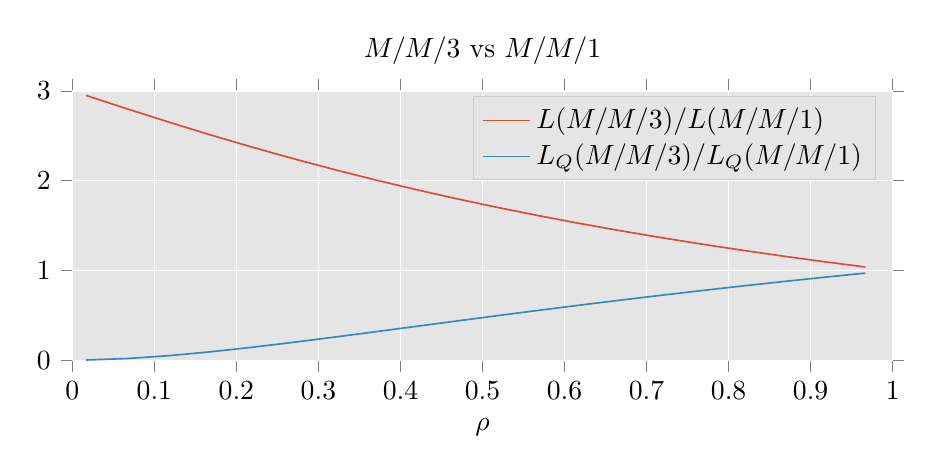
\begin{tikzpicture}

\definecolor{color1}{rgb}{0.203921568627451,0.541176470588235,0.741176470588235}
\definecolor{color0}{rgb}{0.886274509803922,0.290196078431373,0.2}

\begin{axis}[
title={$M/M/3$ vs $M/M/1$},
xlabel={$\rho$},
xmin=0, xmax=1,
ymin=0, ymax=3,
width=12cm,
height=5cm,
tick align=outside,
xmajorgrids,
x grid style={white},
ymajorgrids,
y grid style={white},
axis line style={white},
axis background/.style={fill=white!89.803921568627459!black},
legend cell align={left},
legend style={draw=white!80.0!black, fill=white!89.803921568627459!black},
legend entries={{$\E{L(M/M/3)}/\E{L(M/M/1)}$},{$\E{L_Q(M/M/3)}/\E{L_Q(M/M/1)}$}}
]
\addplot [semithick, color0]
table {%
0.0166666666666667 2.95002015316405
0.0666666666666667 2.80116959064328
0.116666666666667 2.65569956796278
0.166666666666667 2.51515151515152
0.216666666666667 2.38043779440288
0.266666666666667 2.2520325203252
0.316666666666667 2.13010978743284
0.366666666666667 2.01464254952627
0.416666666666667 1.90547263681592
0.466666666666667 1.8023598820059
0.516666666666667 1.7050162643383
0.566666666666667 1.61312938177183
0.616666666666667 1.52637836231238
0.666666666666667 1.44444444444444
0.716666666666667 1.36701781766159
0.766666666666667 1.2938018545632
0.816666666666667 1.22451553720904
0.866666666666667 1.15889464594128
0.916666666666667 1.09669211195929
0.966666666666667 1.03767781622453
};
\addplot [semithick, color1]
table {%
0.0166666666666667 0.00120918984280532
0.0666666666666667 0.0175438596491228
0.116666666666667 0.0488534396809571
0.166666666666667 0.0909090909090909
0.216666666666667 0.1404821280133
0.266666666666667 0.195121951219512
0.316666666666667 0.252978276103714
0.366666666666667 0.31266149870801
0.416666666666667 0.373134328358209
0.466666666666667 0.433628318584071
0.516666666666667 0.493579866461222
0.566666666666667 0.552581261950287
0.616666666666667 0.610343290236291
0.666666666666667 0.666666666666667
0.716666666666667 0.721420210690597
0.766666666666667 0.774524158125915
0.816666666666667 0.82593739250086
0.866666666666667 0.875647668393782
0.916666666666667 0.923664122137404
0.966666666666667 0.970011534025375
};
\end{axis}

\end{tikzpicture}
\end{center}

The  code can be found on \texttt{github} in the \texttt{progs} directory.
\end{solution}
\end{exercise}





\Closesolutionfile{hint}
\Closesolutionfile{ans}

\opt{solutionfiles}{
\subsection*{Hints}
\input{hint}
\subsection*{Solutions}
\input{ans}
}

%\clearpage

%%% Local Variables:
%%% mode: latex
%%% TeX-master: "../queueing_book"
%%% End:
